%*----------- SLIDE -------------------------------------------------------------
\begin{frame}[t]{Introdução} 
    \transdissolve[duration=0.5]
    Um dos pontos importantes na área da robótica é a interação entre os sistemas, e em decorrência ao programa de formação em robótica uma das lacunas será preenchida com o desenvolvimento do desafio 2.5..

    O desafio consiste em:
    %\newline
        \begin{columns}[t]
            \column{.05\linewidth}
            \column{.4\linewidth}
                \begin{enumerate}
                    \item assimilar o conhecimento da interação em robots;
                    \item compreender em profundidade os conceitos de simulação, e o;
                    \item desenvolvimento da liderança em projetos \cite{Mohan2015}.
                \end{enumerate}
            \column{.6\linewidth}
            \begin{center}
            %\centerline{
                \begin{figure}
                    %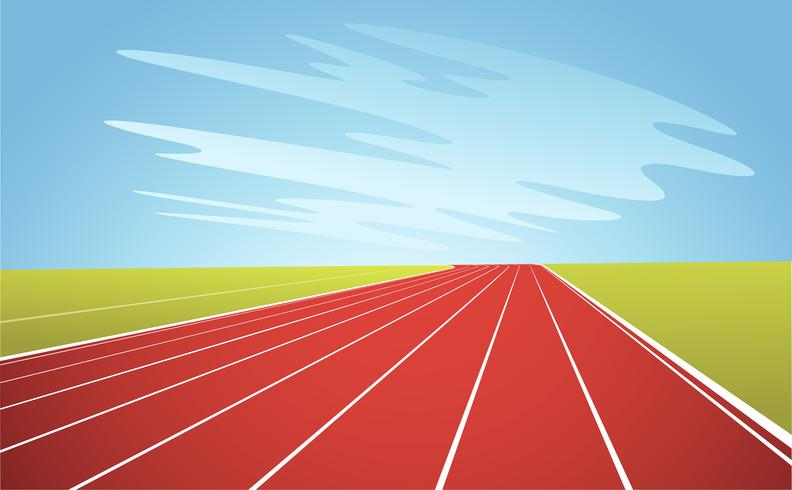
\includegraphics[width=1\textwidth]{pista}
                    \caption{Pista de corrida \cite{agostini2007}}
                    \roundpic[xshift=0cm,yshift=0cm]{2.5cm}{6cm}{pista}
                    %\caption{Pista de corrida \cite{agostini2007}}
                \end{figure}
            %}
            \end{center}
        \end{columns}
%*----------- notes
    \note[item]{Notes can help you to remember important information. Turn on the notes option.}
\end{frame}
%-
%*----------- SLIDE -------------------------------------------------------------
\begin{frame}[c]{Objetivo} 
    \framesubtitle{sub-objetivo}
    \transdissolve[duration=0.5]
   
    \begin{center}
        \Wider{%
        \begin{shaded}
        \begin{center}
            \vspace*{0.5cm}
            \resizebox{!}{0.7cm}{%
                \color{mracula0} O objetivo é ter um objetivo.
            }%
        \end{center}
        \end{shaded}
        }%
    \end{center}
    
   
%*----------- notes
    \note[item]{Notes can help you to remember important information. Turn on the notes option.}
\end{frame}
%-
{
\setbeamertemplate{background}
{
\includegraphics[trim = 0 0 0 0, clip, width = \the\paperwidth, height = \the\paperheight]{marcel-knupfer-37wuETxVwTQ-unsplash.jpg}}
%*----------- SLIDE -------------------------------------------------------------
\begin{frame}[c]{}
    \transboxout[duration=0.5]
    
    \begin{columns}
        \column{.1\textwidth}
        \column{.3\textwidth}
        \column{.53\textwidth}
            \vspace*{-3.5cm}
            \Huge{\textbf{\textcolor{mracula5}{Quando chovia...}}}
    \end{columns}
%*----------- notes
    \note[item]{Notes can help you to remember important information. Turn on the notes option.}
\end{frame}
%-
}
%*----------- SLIDE -------------------------------------------------------------
\begin{frame}[t]{O sistema robótico}
    \transboxout[duration=0.5]
    \framesubtitle{Darwin-OP}
    \begin{columns}
        \column{.1\textwidth}
        \column{.4\textwidth}
            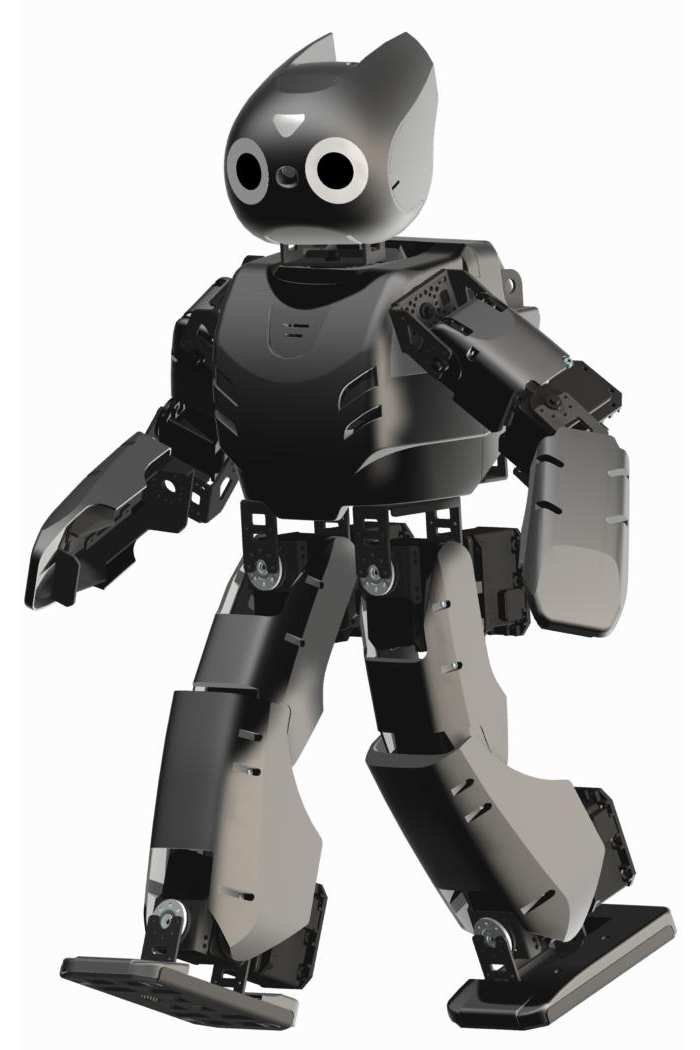
\includegraphics[width=.7\textwidth]{darwin-op}
        \column{.4\textwidth}
            \begin{enumerate}
                \item plataforma antropormórfica Darwin-OP;
                \item 20 DoF\footnote{do inglês, graus de liberdade};
                \item composto de 18 servo-motores;
                \item possui um grande gama de sensores para interação.
            \end{enumerate}
    \end{columns}
 %*----------- notes
    \note[item]{Notes can help you to remember important information. Turn on the notes option.}
\end{frame}
%-
%*----------- SLIDE -------------------------------------------------------------
\begin{frame}[c]{Darwin-OP - overview}
    %\transboxin[duration=1,direction=30]
    \centering

    \includemedia[
      width=0.7\linewidth,
      totalheight=0.39375\linewidth,
      activate=pageopen,
      passcontext, 
      addresource=./Source/movies/Darwin-OP.mp4,
      flashvars={
      source=./Source/movies/Darwin-OP.mp4
      &autoPlay=true
      &Loop=false}
      ]{\fbox{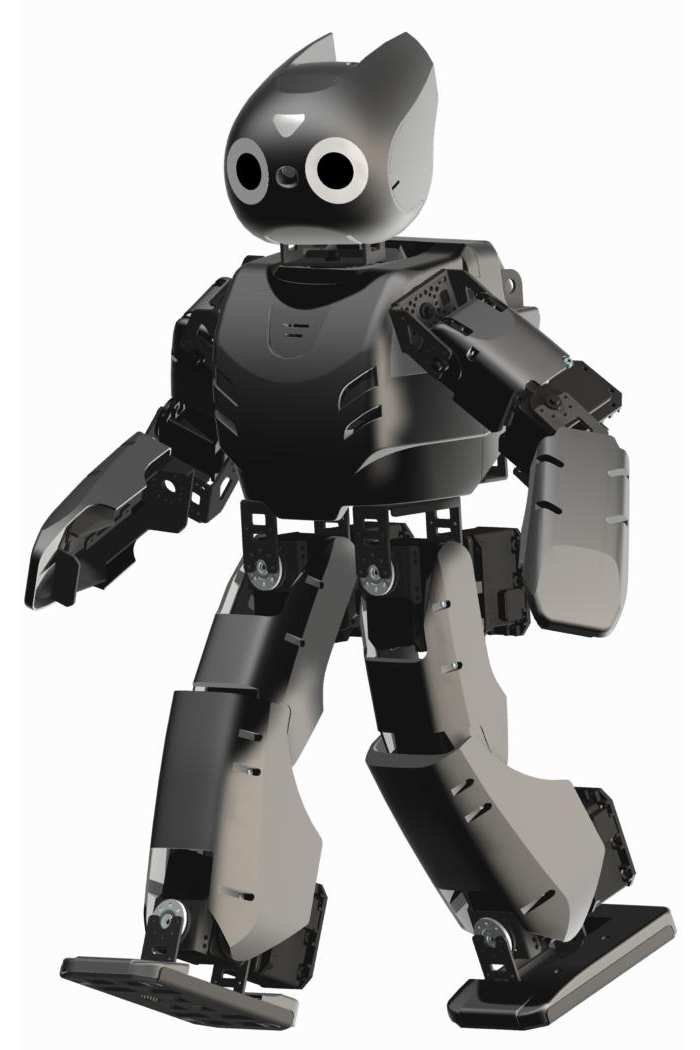
\includegraphics{darwin-op}}}{VPlayer.swf}

%*----------- notes
    \note[item]{Notes can help you to remember important information. Turn on the notes option.}
\end{frame}
%-
%*----------- SLIDE -------------------------------------------------------------
\begin{frame}[t]{O sistema robótico}
    \transboxout[duration=0.5]
    \framesubtitle{Darwin-OP}
    \begin{columns}
        \column{.1\textwidth}
        \column{.4\textwidth}
        \column{.4\textwidth}
    \end{columns}

    \begin{block}{Um bloco de destaque}
        Um exemplo de block.\\
        Oferece um certo destaque.
    \end{block}

    \begin{alertblock}{Um bloco de destaque}
        Um exemplo de alertblock.\\
        Oferece um certo destaque.
    \end{alertblock}

    \begin{exampleblock}{Um bloco de destaque}
        Um exemplo de exampleblock.
    \end{exampleblock}
 %*----------- notes
    \note[item]{Notes can help you to remember important information. Turn on the notes option.}
\end{frame}